% ============================================================
%  HW02 - Domain Testing on EShop
%  Bug Report (LaTeX) - filed via the bug-reporter skill
% ============================================================
\documentclass[11pt,a4paper]{article}

\usepackage[utf8]{inputenc}
\usepackage[T1]{fontenc}
\usepackage[top=2.2cm,bottom=2.2cm,left=2.2cm,right=2.2cm]{geometry}
\usepackage{graphicx}
\usepackage{enumitem}
\usepackage{hyperref}
\hypersetup{colorlinks=true, linkcolor=black, urlcolor=blue}

\newcommand{\code}[1]{\texttt{#1}}

\title{\textbf{Bug Report --- HW02 Domain Testing on EShop}}
\author{SUT: EShop (\url{https://github.com/ttbhanh/eshop-sut})}
\date{2026-07-06}

\begin{document}
\maketitle

% ------------------------------------------------------------
\section*{BUG-001 --- Strong password with a special character is rejected}
\begin{itemize}[leftmargin=*]
  \item \textbf{Feature:} FR-01 \quad \textbf{Technique:} Domain + BVA \quad \textbf{Severity:} Major
  \item \textbf{Description:} The client-side regex requires a whitespace character and
        forbids special characters, so a spec-compliant strong password
        (8+ chars, upper, lower, digit, special) is wrongly rejected.
  \item \textbf{Steps to reproduce:}
    \begin{enumerate}[leftmargin=*]
      \item Open the Register page (\code{/register}).
      \item Enter a valid name and email.
      \item Enter the password \code{Password123!}.
      \item Click ``Dang Ky'' (Register).
    \end{enumerate}
  \item \textbf{Expected:} Registration succeeds and the user is redirected to \code{/login}.
  \item \textbf{Actual:} An error ``Mat khau qua yeu!'' (password too weak) is shown below the
        form; registration does not proceed.
  \item \textbf{GitHub Issue:} \url{https://github.com/dinosauce-285/Software-Testing-G02/issues/1}
\end{itemize}
\begin{figure}[h]\centering
  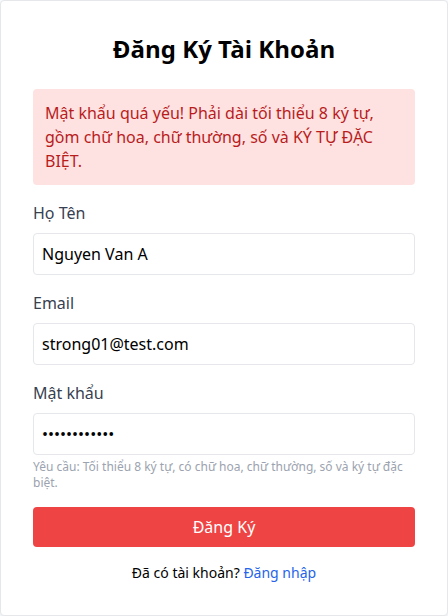
\includegraphics[width=0.8\textwidth]{../figures/bugs/bug_a_01.png}
  \caption{BUG-001 --- strong password rejected on the Register form}
\end{figure}

% APPEND-BELOW

\end{document}
